\documentclass{article}

\usepackage{amsmath}
\usepackage{amssymb}

\usepackage{amsthm}
\theoremstyle{plain}
  \newtheorem{theorem}{Theorem}
  \newtheorem{lemma}[theorem]{Lemma}
  \newtheorem{proposition}[theorem]{Proposition}
  \newtheorem{conjecture}[theorem]{Conjecture}
  \newtheorem{corollary}[theorem]{Corollary}
\theoremstyle{definition}
  \newtheorem{definition}[theorem]{Definition}
  \newtheorem{remark}[theorem]{Remark}
  \newtheorem{example}[theorem]{Example}
  \newtheorem{procedure}[theorem]{Procedure}
  \newtheorem{assumption}[theorem]{Assumption}
\numberwithin{theorem}{section}

\usepackage{color}
\usepackage{graphicx}
\usepackage{geometry}

% fonts
\usepackage{ifluatex}
\ifluatex
  \usepackage[no-math]{fontspec}
\else
  \usepackage[T1]{fontenc}
\fi
\usepackage{newpxtext,newpxmath}

% bibliography
\usepackage[%
  backend=bibtex,bibencoding=ascii,
  style=numeric-comp,
  giveninits=true, uniquename=init, %abbreviate first names
  natbib=true,
  url=true,
  doi=true,
  isbn=false,
  backref=false,
  maxnames=99,
  ]{biblatex}
\addbibresource{references.bib}

\newcommand{\order}{{\mathcal O}}
\newcommand{\todo}[1]{{\Large{\color{red}{#1}}}}


\title{Notes on analysis of some hyperbolized equations}

\begin{document}

\maketitle

\section{General methodology} \label{sec:general}
We use the approach outlined in \cite[Section~5.5]{dafermos2016hyperbolic} to prove regularity of solutions.
Thus, we consider a hyperbolic balance law with source term of the form
\begin{equation}
\begin{aligned}
    \partial_t U + \partial_x G(U) + P(U) &= 0, && x \in \mathbb{R}, t > 0, \\
    U(x, 0) & = U_0(x), && x \in \mathbb{R}.
\end{aligned}
\end{equation}
Assume that $U = 0$ is an equilibrium with $P(0) = 0$, and that there is a convex entropy $\eta$ with associated entropy flux $Q$ satisfying $\eta(0) = 0$, $Q(0) = 0$, $\eta'(0) = 0$, and $Q'(0) = 0$.
We need to check the following properties to obtain global existence of a classical solution for small initial data from \cite[Theorem~5.5.3]{dafermos2016hyperbolic}:
\begin{itemize}
    \item The Hessian $\eta''(U)$ is positive definite ($\eta''(U) = A(U)$ in the notation of \cite[Section~5.5]{dafermos2016hyperbolic}).
    \item The source is dissipative semidefinite, i.e.,
          \begin{equation}
          \label{eq:dissipative_semidefinite}
            \exists a > 0\colon \quad
            \eta'(U) \cdot P(U) \ge a |P(U)|^2.
          \end{equation}
    \item There is a skew-symmetric matrix $K$ such that
          \begin{equation} \label{eq:M}
            M = K G'(0) + \eta''(0) P'(0)
          \end{equation}
          is positive definite (which is implied by the Kawashima
          condition \cite[Section~5.2]{dafermos2016hyperbolic}).
\end{itemize}
If these conditions are satisfied, Theorem 5.5.3 in
\cite[Theorem~5.5.3]{dafermos2016hyperbolic}
gives global existence of a classical solution for initial data
such that $\|U_0\|_{H^\ell}$, $\ell \ge 2$, is sufficiently small.

\todo{Add discussion about scaling symmetry here.}

In Section \ref{sec:viscous-burgers} we 
verify these conditions for the viscous Burgers system \eqref{vbh}.
Next we consider the dissipative p-system.
Unfortunately, for higher-order hyperbolized systems, the condition
\eqref{eq:dissipative_semidefinite} of a dissipative semidefinite source is
not satisfied.  For dispersive systems, there is zero dissipation, while
for dissipative hyperbolized systems, only one variable is directly
dissipated.  The condition \eqref{eq:dissipative_semidefinite} essentially
requires that all variables be directly dissipated.
very strong. Thus it is
not satisfied for KdV-Burgers \cite[Section~3.1.2]{giesselmann2025convergence}
or even the Cahn-Hilliard hyperbolization of Dhaouadi et al.


\section{Viscous Burgers equation} \label{sec:viscous-burgers}
\begin{align}
    u_t + u u_x & = \mu u_{xx}
\end{align}
Hyperbolic approximation:
\begin{subequations} \label{vbh}
\begin{align}
    u_t - \mu v_x + u u_x & = 0 \\
    \tau v_t - u_x & = -v.
\end{align}
For a given value of $\tau$, we refer to \eqref{vbh} as BH($\tau$).
\end{subequations}
For this system we have the entropy
\begin{align} \label{burgers-entropy}
    \eta = \frac{1}{2} \left(u^2 + \mu \tau v^2\right)
\end{align}
with
\begin{align*}
    \eta_t & = u u_t + \mu \tau v v_t \\
    & = \mu u v_x - u^2 u_x + \mu v u_x -\mu v^2 \\
    & = \left( 2 \mu uv - \frac{1}{3}u^3\right)_x - \mu v^2,
\end{align*}
so
\begin{align}
\partial_t \int_{-\infty}^\infty \eta dx & = -\mu \int_\infty^\infty v^2 dx \le 0.
\end{align}


\subsection{Regularity}

\subsubsection{Checking the conditions in Theorem~5.5.3}
Now we apply the approach outlined in Section \ref{sec:general}.  
First note that $(u,v) = (0,0)$ is indeed an equilibrium with $P=0$;
furthermore the entropy (given by \eqref{burgers-entropy} and entropy flux 
(given by $2\mu uv - u^3/3$) and their first derivatives vanish for these values.
We have
\begin{align}
    \eta'' & = \begin{bmatrix}
        1 & 0 \\ 0 & \mu \tau
    \end{bmatrix}
\end{align}
which is positive definite since $\mu \tau >0$.
Next we have
\begin{align}
    \eta' \cdot P & = [u, \mu \tau v] \cdot  \begin{bmatrix} 0 \\ v \end{bmatrix} = \mu \tau v^2 \\
    |P|^2 & = v^2,
\end{align}
so \eqref{eq:dissipative_semidefinite} is satisfied with $a = \mu \tau$.
Then we have
\begin{align}
    G & = \begin{bmatrix} \frac{1}{2} u^2 -\mu v \\ -\tau^{-1} u \end{bmatrix} \\
   G' & = \begin{bmatrix} u & -\mu \\ -\tau^{-1} &  0 \end{bmatrix} \\
   G'(0) & = \begin{bmatrix} 0 & -\mu \\ -\tau^{-1} &  0 \end{bmatrix} \\
   \eta''(0) P'(0) & = \begin{bmatrix} 1 & 0 \\ 0 & \mu \tau \end{bmatrix}
    \begin{bmatrix} 0 & 0 \\ 0 & 1 \end{bmatrix} = 
    \begin{bmatrix} 0 & 0 \\ 0 & \mu \tau \end{bmatrix}.
\end{align}
Taking
\begin{align*}
    K = \begin{bmatrix} 0 & -k \\ k & 0 \end{bmatrix},
\end{align*}
we find that for the matrix \eqref{eq:M},
\begin{align}
    \frac{1}{2}\left(M + M^T\right) & = \begin{bmatrix} \tau^{-1} k & 0 \\ 0 & \mu(\tau-k) \end{bmatrix},
\end{align}
so by taking $0 < k < \tau$, we have that $M$ is positive definite.  Thus all the assumptions
of the theorem are fulfilled, so for small enough initial data $u, v$ we know there exists
a strong solution for all time.

\begin{theorem}
\label{thm:burgers_small_data}
    Let
    $\tau > 0$ and $\ell > 1$.
    Let $U_0 \in L^2(\mathbb{R})$,
    $U_0 \in H^\ell$, and $\|U_0\|_{H^\ell}$ be sufficiently small.
    Then, there is a unique global classical solution $U$ of the Cauchy problem for the BH system \eqref{vbh}.
\end{theorem}
In particular, setting $\tau=1$, Theorem \ref{thm:burgers_small_data} implies that for small
enough initial data there is a unique classical solution  of BH(1).


\subsection{Scaling symmetry}
The system \eqref{vbh} is invariant under the following transformation, for any $\epsilon>0$:
\begin{subequations}
\label{vbh-scaling}
\begin{align}
    \tau & \to \epsilon^2 \tau \\
    x & \to \epsilon x & t & \to \epsilon^2 t \\
    u & \to \epsilon^{-1} u & v & \to \epsilon^{-2} v.
\end{align}
\end{subequations}

\begin{proposition}\label{prop:vbh-scaling}
Consider the Cauchy problem for \eqref{vbh} and let $\epsilon>0$.
Let $q^\epsilon=[u^\epsilon,v^\epsilon]^T$ denote the
solution of BH$(\epsilon^2)$ with initial data
\begin{subequations} \label{bh-scaled-ic}
\begin{align}
    u^\epsilon(x,t=0) & = \epsilon^{-1} u_0(x/\epsilon) \\
    v^\epsilon(x,t=0) & = \epsilon^{-2} v_0(x/\epsilon)
\end{align}
\end{subequations}
Then we have
\begin{subequations} \label{bh-scaled-ic-2}
\begin{align}
    u^{\epsilon}(x,t) & = \epsilon^{-1} u^1(x/\epsilon, t/\epsilon^2) \\
    v^{\epsilon}(x,t) & = \epsilon^{-2} v^1(x/\epsilon, t/\epsilon^2)
\end{align}
\end{subequations}
\end{proposition}
Note that when well-prepared data is used (i.e. $v=u_x, w = v_x$) for some value of
$\epsilon$, the initial data \eqref{scaled-ic} is well-prepared for any value of $\epsilon$.


\subsubsection{Applying the scaling symmetry}
By using the scaling symmetry \eqref{vbh-scaling}, we can also obtain a similar result for large initial data, but small $\tau$.
\begin{theorem}
\label{thm:bh_small_tau}
    Let
    $U_0 \in L^2(\mathbb{R})$ and
    $U_0 \in H^2$.
    Then, there exists $\tau > 0$ sufficiently small such that
    there is a unique global classical solution $U$ of the Cauchy problem for the BH($\tau$) system \eqref{vbh}
    with initial data $U_0$.
\end{theorem}
\begin{proof}
%    In order to apply Theorem \ref{thm:small_data} we should fix $\tau_1, \tau_2$; for concreteness
%    let us take $\tau_1=\tau_2=1$.
    Let $U^\epsilon(x,t)$ denote the solution of
    BH$(\epsilon^2)$ with the fixed initial data $u_0(x),v_0(x)$.  From \eqref{bh-scaled-ic-2}
    we have that this is equivalent to the solution of BH(1) with initial data
    \begin{align*}
        u^1(x,t=0) & = \epsilon u_0(\epsilon x, \epsilon^2 t) \\
        v^1(x,t=0) & = \epsilon^2 v_0(\epsilon x, \epsilon^2 t).
    \end{align*}
    Thus $u^1 \propto \epsilon$, $v^1\propto \epsilon^2$, $\partial_x u^1 \propto \epsilon^2$,
    $\partial_x v^1 \propto \epsilon^3$.  By taking $\epsilon$ small enough, 
    we can make $\|U^1_0\|_{H^\ell}$ small enough to apply Theorem \ref{thm:burgers_small_data}.
\end{proof}


\section{Dissipative p-system (p-system with damping) with a nonlinear flux}

We consider here the following genuinely non-linear generalization of the viscous Burgers' equation
\begin{equation}\label{vbh-nl}
u_t + f(u)_x =  (p'(u) u_x)_x
\end{equation}
where we assume that 
\begin{equation}\label{vbh-nl-p}
p'(u) >0\,, \forall u\ge 0.
\end{equation}
Let 
\begin{equation}\label{vbh-nl1}
N(u) = \int p(u)  du\,,\quad
\Pi(u) = \int p(u)f'(u) du\,. 
\end{equation}
We consider now the relaxation approximation 
\begin{equation}\label{psys-nl1}
\begin{aligned}
u_t + &  f(u)_x - v_x =0\\
\tau v_t -& p(u)_x = -v
\end{aligned}
\end{equation}
whose eigenvalues are now $(\lambda_1,\lambda_2)=(f'(u)/2 - \sqrt{f'(u)^2  + 4 p'(u)/\tau}/2,\,f'(u)/2 + \sqrt{f'(u)^2  + 4 p'(u)/\tau}/2)$.
The system admits and entropy/entropy flux which is given by
$$
\eta(U) = N(u) +  \tau\dfrac{v^2}{2}\,,\quad
F = \Pi(u) - p(u)v
$$
for which we have 
$$
\eta'(U) =  [p(u),\,  \tau v]^T\,,\;\; \eta''(U) = \left[\begin{array}{cc}
p'(u)&  0\\
0 & \tau
\end{array}
\right]>0
$$
For a given value of $\tau$, we refer to \eqref{vbh-nl-p} as PH($\tau$).

\subsection{Regularity}


We proceed as before. We can see that in this case
$$
G'=\left[\begin{array}{cc}
f'(u)&  -1\\
p'(u)/\tau & 0
\end{array}\right]\Rightarrow G(0)'=\left[\begin{array}{cc}
f'(0)&  -1\\
-p'(0)/\tau & 0
\end{array}\right].
$$
We can also check that 
$$
\eta''(0)P'(0) = \left[\begin{array}{cc}
0&  0\\
0 &  \tau
\end{array}\right]
$$
We now take
\begin{align*}
    K = \begin{bmatrix} 0 & -k \\ k & b \end{bmatrix},
\end{align*}
so that
$$
M=KG'(0) + \eta''(0)P'(0) = 
  \left[\begin{array}{cc}
\dfrac{kp'(0)}{\tau} &  0\\
kf'(0) -\dfrac{bp'(0)}{\tau} &   \tau -k
\end{array}\right] 
$$
So  the matrix \eqref{eq:M} is 
$$
\dfrac{1}{2}(M+M^T) =\dfrac{1}{2}\left[\begin{array}{cc}
2\dfrac{kp'(0)}{\tau} &  kf'(0) -\dfrac{bp'(0)}{\tau} \\
kf'(0) -\dfrac{bp'(0)}{\tau} &   2(\tau -k)
\end{array}\right] 
$$
We take now $k\in (0,\tau)$, and choose
$$
b=  \dfrac{\tau k f'(0)}{p'(0)}
$$
so that the resulting matrix is positive definite.  Thus all the assumptions of the theorem are fulfilled, and for small enough initial data $u, v$ we know there exists
a strong solution for all time.

\begin{theorem}
\label{thm:Psys_small_data}
    Let
    $\tau > 0$ and $\ell > 1$.
    Let $U_0 \in L^2(\mathbb{R})$,
    $U_0 \in H^\ell$, and $\|U_0\|_{H^\ell}$ be sufficiently small.
    Then, there is a unique global classical solution $U$ of the Cauchy problem for the PH system \eqref{psys-nl1}.
\end{theorem}
In particular, setting $\tau=1$, Theorem \ref{thm:burgers_small_data} implies that for small
enough initial data there is a unique classical  solution of PH(1).

\subsection{Scaling symmetry}








\section{Some examples not verifying the regularity conditions}

\subsection{Hyperbolized forms of the KdV equation with viscosity}

\begin{align}
    u_t + u u_x + u_{xxx} = \mu u_{xx}
\end{align}
We study here different hyperbolic approximations of this equation. 
A first  hyperbolic approximation taken from \cite{giesselmann2025convergence} reads  
\begin{subequations} \label{vkdvh1}
\begin{align}
    u_t + u u_x  + w_x & = 0 \\
    \tau v_t   - v_x  & = -w -\mu v\\
        \tau w_t +  u_x & = v
%            \tau z_t - u_x & = -z 
\end{align}
\end{subequations}
This system has eigenvalues $(\lambda_1,\; \lambda_2,\;\lambda_3)=(u/2 - \sqrt{u^2+4/\tau}/2, -1/\tau, u/2+ \sqrt{u^2+4/\tau}/2)$.
The entropy is easily shown to be $\eta(U) = u^2/2 + \tau (v^2+w^2)/$, so we have 
$$
\eta'(U)= [u\;, \tau v\;, \tau w]^T\;,\quad 
\eta''(U) =  \text{diag}(1,\tau,\tau) >0.
$$
The entropy flux is obtained from
$$
F_x =u (u u_x  + w_x) - v v_x + wu_x = ( u^3/2 - v^2/2  + uw )_x\Rightarrow F = u^3/2 - v^2/2  + uw.
$$
The source entropy production is for this system
$$
\eta'(U)\cdot P(U) = [u\;, \tau v\;, \tau w] [0\;, w +\mu v\;, -v]^T = \tau \mu v^2  
$$
We now need to check that this term can be used to bound from above the the squared norm of the source term?
So we need to find some constant $a$ such that  
$$
  a \tau \mu   v^2 \stackrel{?}{\ge} \|P(U)\|^2 = v^2 + (w +\mu v)^2 
$$
which is in general not true since the $w$ terms on the right hand side cannot be controlled.\\



As an alternative let us now consider the approximation
\begin{subequations} \label{vkdvh2}
\begin{align}
    u_t + u u_x  + w_x -\mu w & = 0 \\
    \tau v_t - v_x & = -w\\
        \tau w_t +  u_x & = v
%            \tau z_t - u_x & = -z 
\end{align}
\end{subequations} 
This system is hyperbolic with  same eigenvalues  and same entropy and entropy flux as the previous. 
We can see that  the source entropy production is
$$
\eta'(U)\cdot P(U) = [u\;, \tau v\;, \tau w] [-\mu w\;, w\;, -v]^T =- \mu u w
$$
which is unfortunately unsigned and again does not allow to apply Daferrmos' criterion.\\

 

Finally we  study   the augmented system
\begin{subequations} \label{vkdvh3}
\begin{align}
    u_t +  u u_x  + w_x -\mu z_x & = 0 \\
    \tau v_t - v_x & = -w\\
        \tau w_t  + u_x  & = v
            \tau z_t - u_x & = -z 
\end{align}
\end{subequations}
We have now the eigenvalues $(\lambda_1,\;\lambda_2,\;\lambda_3,\;\lambda_4)=(u/2 - \sqrt{u^2+(1+\mu)2/\tau}/2, -1/\tau, 0 , u/2 + \sqrt{u^2+(1+\mu)2/\tau}/2)$.
The entropy is now $\eta(U) =u^2/2 + \tau v^2/2 + \tau w^2/2 +\tau  \mu  z^2/2$ and the entropy flux is obtained from
$$
F_x = u( u u_x  + w_x -\mu z_x) - vv_x +wu_x -\mu z u_x  \Rightarrow  F=u^3/3  -v^2/2 + uw -\mu uz.
$$
We also have 
$$
\eta'(U)= [u\;, \tau v\;, \tau w\;, \tau\mu z]^T\;,\quad 
\eta''(U) =  \text{diag}(1,\tau,\tau,\tau \mu) >0.
$$
Let us now check the  sign  condition
$$
\eta'(U)\cdot P(U) = [u\;, \tau v\;, \tau w\;, \tau\mu z] [ 0,\; w,\; -v,\; z ]^T = \tau \mu z^2 ,
$$
which has the correct sign. We need now to verify the upper bound  condition :
$$
  a \tau \mu   v^2 \stackrel{?}{\ge} \|P(U)\|^2 = w^2 + v^2 + z^2 .
$$
This cannot be true in general as we cannot control the $w^2 + z^2$ term.

%
%
%\begin{subequations} \label{vbh0}
%\begin{align}
%    u_t + u u_x  + w_x -\mu z_x & = 0 \\
%    \tau v_t - v_x & = -w\\
%        \tau w_t +  u_x & = v\\
%            \tau z_t - u_x & = -z 
%\end{align}
%\end{subequations}
%For this system we have the entropy
%\begin{align}
%    \eta = \frac{1}{2} \left(u^2 + \mu \tau v^2\right)
%\end{align}
%with
%\begin{align*}
%    \eta_t & = u u_t + \mu \tau v v_t \\
%    & = \mu u v_x - u^2 u_x + \mu v u_x -\mu v^2 \\
%    & = \left( 2 \mu uv - \frac{1}{3}u^3\right)_x - \mu v^2,
%\end{align*}
%so
%\begin{align}
%\partial_t \int_{-\infty}^\infty \eta dx & = -\mu \int_\infty^\infty v^2 dx \le 0.
%\end{align}
%


\subsection{Cahn-Hilliard equations}

This section considers the Cahn-Hilliard equations given by

\begin{subequations} \label{CaHi}
\begin{align}
c_t  & -  h_{xx} +\gamma c_{xxxx} =0\\
h &=h(c) = \dfrac{dg(c)}{dc}
\end{align}
\end{subequations}
with $g(c)$ the so-called  double-well potential, and $\sqrt{\gamma}$   the (given, small) characteristic length of  the phase transition layer.
We consider the hyperbolic reformulation by \cite{dhaouadi25} which can be written as (using the appropriate scaling parameters)
\begin{subequations} \label{hCaHi}
\begin{align}
c_t  &  +\dfrac{1}{\tau} q_x =0\\
q_t  &  + h_x +\alpha c_x- \alpha\varphi_x = - \dfrac{1}{\tau} q\\
w_t  &  -  \gamma p_x =  -\alpha (\varphi-c)\\
p_t  &  -   \dfrac{1}{\beta} w_x =0\\
\varphi_t &  =   \dfrac{1}{\beta} w 
\end{align}
\end{subequations}
The reference shows the asymptotic consistency of this model in the scaling 
$$\tau = \gamma^2,\;, \alpha=\gamma^{-1} = \tau^{-1/2},\; \beta =\gamma^2 = \tau,$$ 
which would lead to  the  (correctly) scaled equations
\begin{subequations} \label{hCaHi1}
\begin{align}
c_t  &  +\dfrac{1}{\gamma^2} q_x =0\\
q_t  &  + h_x +\dfrac{1}{\gamma} c_x- \dfrac{1}{\gamma}\varphi_x =  \dfrac{1}{\gamma^2} q\\
w_t  &  -  \gamma p_x = - \dfrac{1}{\gamma} (\varphi-c)\\
p_t  &  -   \dfrac{1}{\gamma^2} w_x =0\\
\varphi_t &  =   \dfrac{1}{\gamma^2} w 
\end{align}
\end{subequations}
The hyperbolicity of the system is studied in \cite{dhaouadi25}, where the authors also show the existence of the entropy
$$
\eta(U) = g +\dfrac{\gamma}{2}p^2 + \dfrac{1}{2\gamma } (c-\varphi)^2  + \dfrac{1}{2\gamma^2}w^2 +  \dfrac{1}{2\gamma^2}q^2
$$
with
$$
\eta'(U)= [h+ \dfrac{1}{\gamma } (c-\varphi),\,  \dfrac{1}{\gamma^2 }q,\,  \dfrac{1}{\gamma^2 }w,\, \gamma p,\,    -\dfrac{1}{\gamma } (c-\varphi) ]^T\;,\quad 
\eta''(U) =   \left[\begin{array}{ccccc}
h' +\dfrac{1}{\gamma} &0&0&0&-\dfrac{1}{\gamma} \\
0 & \dfrac{1}{\gamma} &0&0&0\\
0 & 0&\dfrac{1}{\gamma} &0&0\\
0 & 0&0& \gamma &0\\
-\dfrac{1}{\gamma} & 0&0& 0 &\dfrac{1}{\gamma} \\
\end{array}
\right]
$$
with the Hessian always positive if $h'\ge 0$. The Dafermos' condition on the entropy production  reads for this system
$$
\begin{aligned}
\eta'(U)^T\cdot P(U) = &[h+ \dfrac{1}{\gamma } (c-\varphi),\,  \dfrac{1}{\gamma^2 }q,\,  \dfrac{1}{\gamma^2 }w,\, \gamma p,\,    -\dfrac{1}{\gamma } (c-\varphi) ]
[0,\,  \dfrac{1}{\gamma^2 }q,\,  \dfrac{1}{\gamma }(\varphi-c),\, 0,\,    -\dfrac{1}{\gamma^2 } w ]^T\\= &
 \dfrac{1}{\gamma^4 }q^2 
\end{aligned}
$$
which  cannot be used to control the full norm $\|P(U)\|^2 = q^2/\gamma^4 +(c-\varphi)^2/\gamma^2 +w^2/\gamma^4 $, so does not verify all the conditions of Dafermos' Theorem.



\section{KdVH}

The KdVH system is
\begin{subequations} \label{kdvh}
\begin{align}
    u_t + uu_x + w_x & = 0 \\
    \tau_1 v_t - v_x & = -w \\
    \tau_2 w_t + u_x & = v.
\end{align}
\end{subequations}
When it is necessary to specify the values of $\tau_1, \tau_2$ we will
refer to KdVH$(\tau_1,\tau_2)$.

\subsection{Scaling symmetry}
The system \eqref{kdvh} is invariant under the following
transformation, for any $\epsilon>0$:
\begin{subequations}
\label{eq:scaling}
\begin{align}
    \tau_1 & \to \epsilon^2 \tau_1 & \tau_2 & \to \epsilon^4 \tau_2 \\
    x & \to \epsilon x & t & \to \epsilon^3 t \\
    u & \to \epsilon^{-2} u & v & \to \epsilon^{-3} v \\
    w & \to \epsilon^{-4} w.
\end{align}
\end{subequations}

\begin{proposition}\label{prop:scaling}
Consider the Cauchy problem for \eqref{kdvh} and let $\epsilon>0$.
Let $q^\epsilon=[u^\epsilon,v^\epsilon,w^\epsilon]^T$ denote the
solution of KdVH$(\epsilon^2,\epsilon^4)$ with initial data
\begin{subequations} \label{scaled-ic}
\begin{align}
    u(x,t=0) & = \epsilon^{-2} u_0(x/\epsilon) \\
    v(x,t=0) & = \epsilon^{-3} v_0(x/\epsilon) \\
    w(x,t=0) & = \epsilon^{-4} w_0(x/\epsilon).
\end{align}
\end{subequations}
Then we have
\begin{subequations}
\begin{align}
    u^{\epsilon}(x,t) & = \epsilon^{-2} u^1(\epsilon^{-1} x, \epsilon^{-3} t) \\
    v^{\epsilon}(x,t) & = \epsilon^{-3} v^1(\epsilon^{-1} x, \epsilon^{-3} t) \\
    w^{\epsilon}(x,t) & = \epsilon^{-4} w^1(\epsilon^{-1} x, \epsilon^{-3} t).
\end{align}
\end{subequations}
\end{proposition}
Note that when well-prepared data is used (i.e. $v=u_x, w = v_x$) for some value of
$\epsilon$, the initial data \eqref{scaled-ic} is well-prepared for any value of $\epsilon$.

\subsection{Asymptotic expansion}
We assume there exist power series for $u, v, w$ in terms of $\tau$:
\begin{align}
    u & = u^0 + \tau u^1 + \tau^2 u^2 + \cdots
    v & = v^0 + \tau v^1 + \tau^2 v^2 + \cdots
    w & = w^0 + \tau w^1 + \tau^2 w^2 + \cdots
\end{align}
Inserting these into \eqref{kdvh} and collecting terms we obtain the following.

$\order(\tau^0)$:
\begin{subequations}
\begin{align}
    v^0 & = u^0_x \\
    w^0 & = v^0_x \\
    u^0 + u^0 u^0_x + w^0_x & = 0.
\end{align}
\end{subequations}

(fill in the rest of the derivation here)

Finally, we obtain (KdVH1)
\begin{align} \label{kdvh1}
    u_t + u u_x + u_{xxx} - \tau\left(u-u_{xx}  \right)_{xxt} - \tau^2\left(2u-u_{xx}\right)_{xxxtt} & = \order(\tau^3).
\end{align}
It would be straightforward to obtain additional terms in this equation if we think that would
be useful.
The expansion including only the $O(\tau)$ term was given in \cite[eq.~(14)]{besse2022perfectly}.

\subsection{Characteristic form}
For the homogeneous hyperbolic part of KdVH, the eigenvalues of the flux Jacobian are
\begin{align}
    \lambda_0 & = -1/\tau_1 \\
    \lambda_\pm & = \frac{u}{2} \pm \frac{\sqrt{u^2 +4/\tau_2}}{2}.
\end{align}
The Riemann invariants are given by $v$ and
\begin{align}
\nu_\pm & = w + \frac{u}{2} \lambda_\pm \pm \frac{\log(\lambda_+)}{\tau_2}.
\end{align}
Note that the system has two genuinely nonlinear fields and one linearly
degenerate field.

In terms of these quantities, the full system \eqref{kdvh} can be written
\begin{subequations}
\begin{align}
    v_t - \frac{1}{\tau_1} v_x & = -\frac{1}{\tau_1} w \\
    (\nu_\pm)_t + \lambda_\pm (\nu_\pm)_x & = \frac{1}{\tau_2} v.
\end{align}
\end{subequations}
It may be useful to express $w$ in terms of the Riemann invariants
in order to better understand this system.




\subsection{Regularity results}
{\bf Note: the analysis in this section is based on a theorem in the 2nd
edition of Dafermos' book, whose proof seems to be incorrect.  Thus it
seems that these results are not valid.}

Following Dafermos \cite[Section~5.2]{dafermos2010hyperbolic}, we write the KdVH system \eqref{kdvh} as
\begin{equation}\label{eq:kdvh_con}
\begin{aligned}
    \partial_t U + \partial_x G(U) + P(U) &= 0, && x \in \mathbb{R}, t > 0, \\
    U(x, 0) &= U_0(x), && x \in \mathbb{R},
\end{aligned}
\end{equation}
where $U = (u, v, w)^T$, the flux function is
\begin{equation}
    G(U) = \left( \frac{1}{2} u^2 + w, -\tau_1^{-1} v, \tau_2^{-1} u \right)^T,
\end{equation}
and the source term is
\begin{equation}
    P(U) = \left( 0, \tau_1^{-1} w, -\tau_2^{-1} v \right)^T.
\end{equation}
In their notation, $\overline{U} = 0$ is indeed a constant equilibrium.
Furthermore,
\begin{equation}
    \eta(U) = \frac{1}{2} u^2 + \frac{\tau_1}{2} v^2 + \frac{\tau_2}{2} w^2
\end{equation}
is a uniformly convex entropy satisfying
\begin{equation}\label{eq:kdvh_entropyeq}
    \partial_t \eta(U) + \partial_x Q(U) + \underbrace{\eta'(U) P(U)}_{= 0} = 0,
\end{equation}
where
\begin{equation}
    Q(U) = \frac{1}{6} u^3 + u w - \frac{1}{2} v^2
\end{equation}
is the associated entropy flux. Note that
\begin{equation}
    P'(U) = \begin{pmatrix}
        0 & 0 & 0 \\
        0 & 0 & \tau_1^{-1} \\
        0 & -\tau_2^{-1} & 0
    \end{pmatrix}.
\end{equation}
Thus, the source term $P$ is not strongly dissipative in the sense of \cite[Section~5.2, p.~109]{dafermos2010hyperbolic}.
However, the assumption \cite[(5.2.12)]{dafermos2010hyperbolic} is satisfied for $\tau_1 \ne 0 \ne \tau_2$, i.e.,
\begin{equation}
    P'(\overline{U}) R_i(\overline{U}) \ne 0, \qquad i \in \{1, 2, 3\},
\end{equation}
since the eigenvectors $R_i$ of the flux Jacobian $G'(U)$ are \cite{besse2022perfectly}
\begin{equation}
    \begin{pmatrix}
        0 \\ 1 \\ 0
    \end{pmatrix},
    \quad
    \begin{pmatrix}
        *_+ \\ 0 \\ 1
    \end{pmatrix},
    \quad
    \begin{pmatrix}
        *_- \\ 0 \\ 1
    \end{pmatrix},
\end{equation}
where $*_\pm$ are nonzero values that are not required for the following argument.
Thus, \cite[Theorem~5.2.1]{dafermos2010hyperbolic} applies, and we obtain the following result.
\begin{theorem}
\label{thm:small_data}
    Let
    $\tau_1, \tau_2 > 0$ and $\ell > 1$.
    Let $U_0 \in L^2(\mathbb{R})$,
    $\nabla U_0 \in H^\ell$, and
    $\|\nabla U_0\|_{H^\ell}$ be sufficiently small.
    Then, there is a unique global classical solution $U$ of the Cauchy problem for the KdVH system \eqref{kdvh}.
\end{theorem}

By using the scaling symmetry \eqref{eq:scaling}, we can also obtain a similar result for large initial data, but small $\tau_1, \tau_2$.
\begin{theorem}
\label{thm:small_tau}
    Let
    $U_0 \in L^2(\mathbb{R})$ and
    $\nabla U_0 \in H^1$.
    Then, there are $\tau_1, \tau_2 > 0$ sufficiently small such that
    there is a unique global classical solution $U$ of the Cauchy problem for the KdVH system \eqref{kdvh}.
\end{theorem}
\begin{proof}
%    In order to apply Theorem \ref{thm:small_data} we should fix $\tau_1, \tau_2$; for concreteness
%    let us take $\tau_1=\tau_2=1$.
    Let $u_0^\epsilon(x,t)$ denote the solution of
    KdVH$(\epsilon^2,\epsilon^4)$ with the fixed initial data $u_0(x)$.  By
    Proposition \ref{prop:scaling}, $u_0^\epsilon(x,t)$ is identical, up to
    rescaling $x$ and $t$, to the solution of KdVH(1,1) but with initial data
    $\tilde{u} = \epsilon^2 u_0(\epsilon x)$.  Thus $\partial_x u_0$ scales like $\epsilon^3$,
    so
    \begin{equation}
        \| \nabla u_0 \|_{L^2} \mapsto \epsilon^{3/2} \| \nabla u_0 \|_{L^2}, \qquad
        | \nabla u_0 |_{H^1} \mapsto \epsilon^{1/2} | \nabla u_0 |_{H^1}.
    \end{equation}
    The other components $v_0, w_0$ behave in the same way if they are initialized with well-prepared initial data, i.e., $v_0 = \partial_x u_0$ and $w_0 = \partial_{xx} u_0$.
    Thus, we can choose $\epsilon$ (and consequently $\tau_1$ and $\tau_2$) sufficiently small such that $\|\nabla U_0\|_{H^1}$ is sufficiently small after the scaling to apply Theorem~\ref{thm:small_data}.
\end{proof}

This sheds more light on how the convergence of (possibly discontinuous, weak entropy) solutions of KdVH to smooth solutions of KdV as $\tau_1, \tau_2 \to 0$ \cite[Theorem~3.2]{giesselmann2025convergence} happens.
Indeed, for given initial data, there are critical thresholds for $\tau_1, \tau_2$ below which there are only classical solutions on KdVH.

Using the scaling symmetry \eqref{eq:scaling} the other way round, we notice that KdVH may have discontinuous solutions for any $\tau_1, \tau_2 > 0$ as long as the initial data are sufficiently big (in the sense of $\| U_0 \|_{H^\ell}$ not being small).


\subsection{Discontinuous solutions}


The conservative form \eqref{eq:kdvh_con} of KDVH system, as well as the entropy balance \eqref{eq:kdvh_entropyeq} can be used to characterize
discontinuous solutions which may appear when the initial data  does not satisfy conditions of theorems 4.1 and 4.2.  If existing,  discontinuities of \eqref{eq:kdvh_con}
travelling at  speed $C$  should verify the classical conditions  (add ref ?)
\begin{equation}\label{eq:shock-conditions}
\begin{aligned}
-C [\![ U]\!] & +  [\![ G]\!] =0 \\[5pt]
-C [\![ \eta]\!] & +  [\![ Q]\!] = \le 0
\end{aligned}
\end{equation}
where  the equal sign in the second condition applies to  linearly degenerate  discontinuities. The first above provides the following system:
\begin{equation}
\begin{aligned}
-C [\![ u]\!] & +  [\![  \dfrac{u^2}{2} + w]\!] =0 \\[5pt]
-C [\![ v]\!] & -\dfrac{1}{\tau_1}  [\![   v]\!] =0 \\[5pt]
-C [\![ w]\!] & +\dfrac{1}{\tau_2}  [\![  u]\!] =0
\end{aligned}
\end{equation}
From this system we can  deduce the existence of two families of solutions. To see this, we recast the above identities as
\begin{equation}\label{eq:RH}
\begin{aligned}
-  [\![ u]\!]  &( C- { \overline u} -\dfrac{1}{\tau_2 C}    )=0   \\[5pt]
-  [\![ v]\!]  &( C+ \dfrac{1}{\tau_1}  )=0   \\[5pt]
\tau_2 C  [\![ w]\!] & =   [\![ u]\!]
\end{aligned}
\end{equation}
with $\overline{(\cdot)}$ denoting the arithmetic average between the right and left states.

The first two  relations provide two different compatibility conditions.
One of these only allows for  discontinuities of $v$, and  it requires  the shock speed to be given by the speed of the linearly degenerate Riemann invariant $\nu_0=v$:
\begin{equation}
  C = - \dfrac{1}{\tau_1}.
\end{equation}
 If this is the case,   from the first and last in \eqref{eq:RH}   we deduce $[\![ u]\!] =[\![ w]\!] =0 $. This is essentially a contact discontinuity  moving at speed $C=\lambda_0$.
 Being a linearly degenerated discontinuity, we expect the second in \eqref{eq:shock-conditions} to hold with an equal sign. This can be easily verified:
\begin{equation}
-C [\![\eta ]\!]  +  [\![ Q ]\!] =  - (\tau_1 C + 1) {\overline  v }  [\![ v ]\!] = 0
\end{equation}
for any value of the initial data since $\tau_1 C + 1$ vanishes. \\

The second family of discontinuities is genuinely nonlinear and associated to the compatibility condition
\begin{equation}
C- { \overline u} -\dfrac{1}{\tau_2 C} =0 \Rightarrow   C^2 - { \overline u} C  -\dfrac{1}{\tau_2 } =0.
\end{equation}
The above quadratic equation has    roots given by
\begin{equation}
C_{\pm} = \dfrac{\overline u}{2} \pm \dfrac{1}{2} \sqrt{{\overline u}^2 +\dfrac{4}{\tau_2} }
\end{equation}
which are associated to the genuinely nonlinear fields $\nu_{\pm}$. When $C$ is given by one of the above roots, one easily sees that the previous compatibility relation implies $ [\![ v ]\!]=0$.  For these discontinuities we expect the condition on the entropy in \eqref{eq:shock-conditions} to be an inequality. This needs to be checked and may provide
admissibility conditions for the initial data. We thus write
\begin{equation}
\begin{aligned}
-C [\![\eta ]\!]  & +  [\![ Q ]\!] =  \text{to be continued ..}
\end{aligned}
\end{equation}







\todo{TODO: Check well-posedness results for KdV}

\todo{TODO: Can we reverse-engineer relative energy convergence results to show well-posedness of KdV using this?}


\subsection{Some numerical results}

The results currently included here are computed using a 1st-order HLL solver.  It should be
kept in mind that this is quite dissipative so longer-time solutions will not be accurate.

For all of these solutions the initial condition is
\begin{align}
    u(x,t=0) = 2 \exp(-x^2/50).
\end{align}

In Figure \ref{fig:convergence}, we observe visual convergence to the KdV solution as
$\tau$ is decreased.

\begin{figure}
\centering
    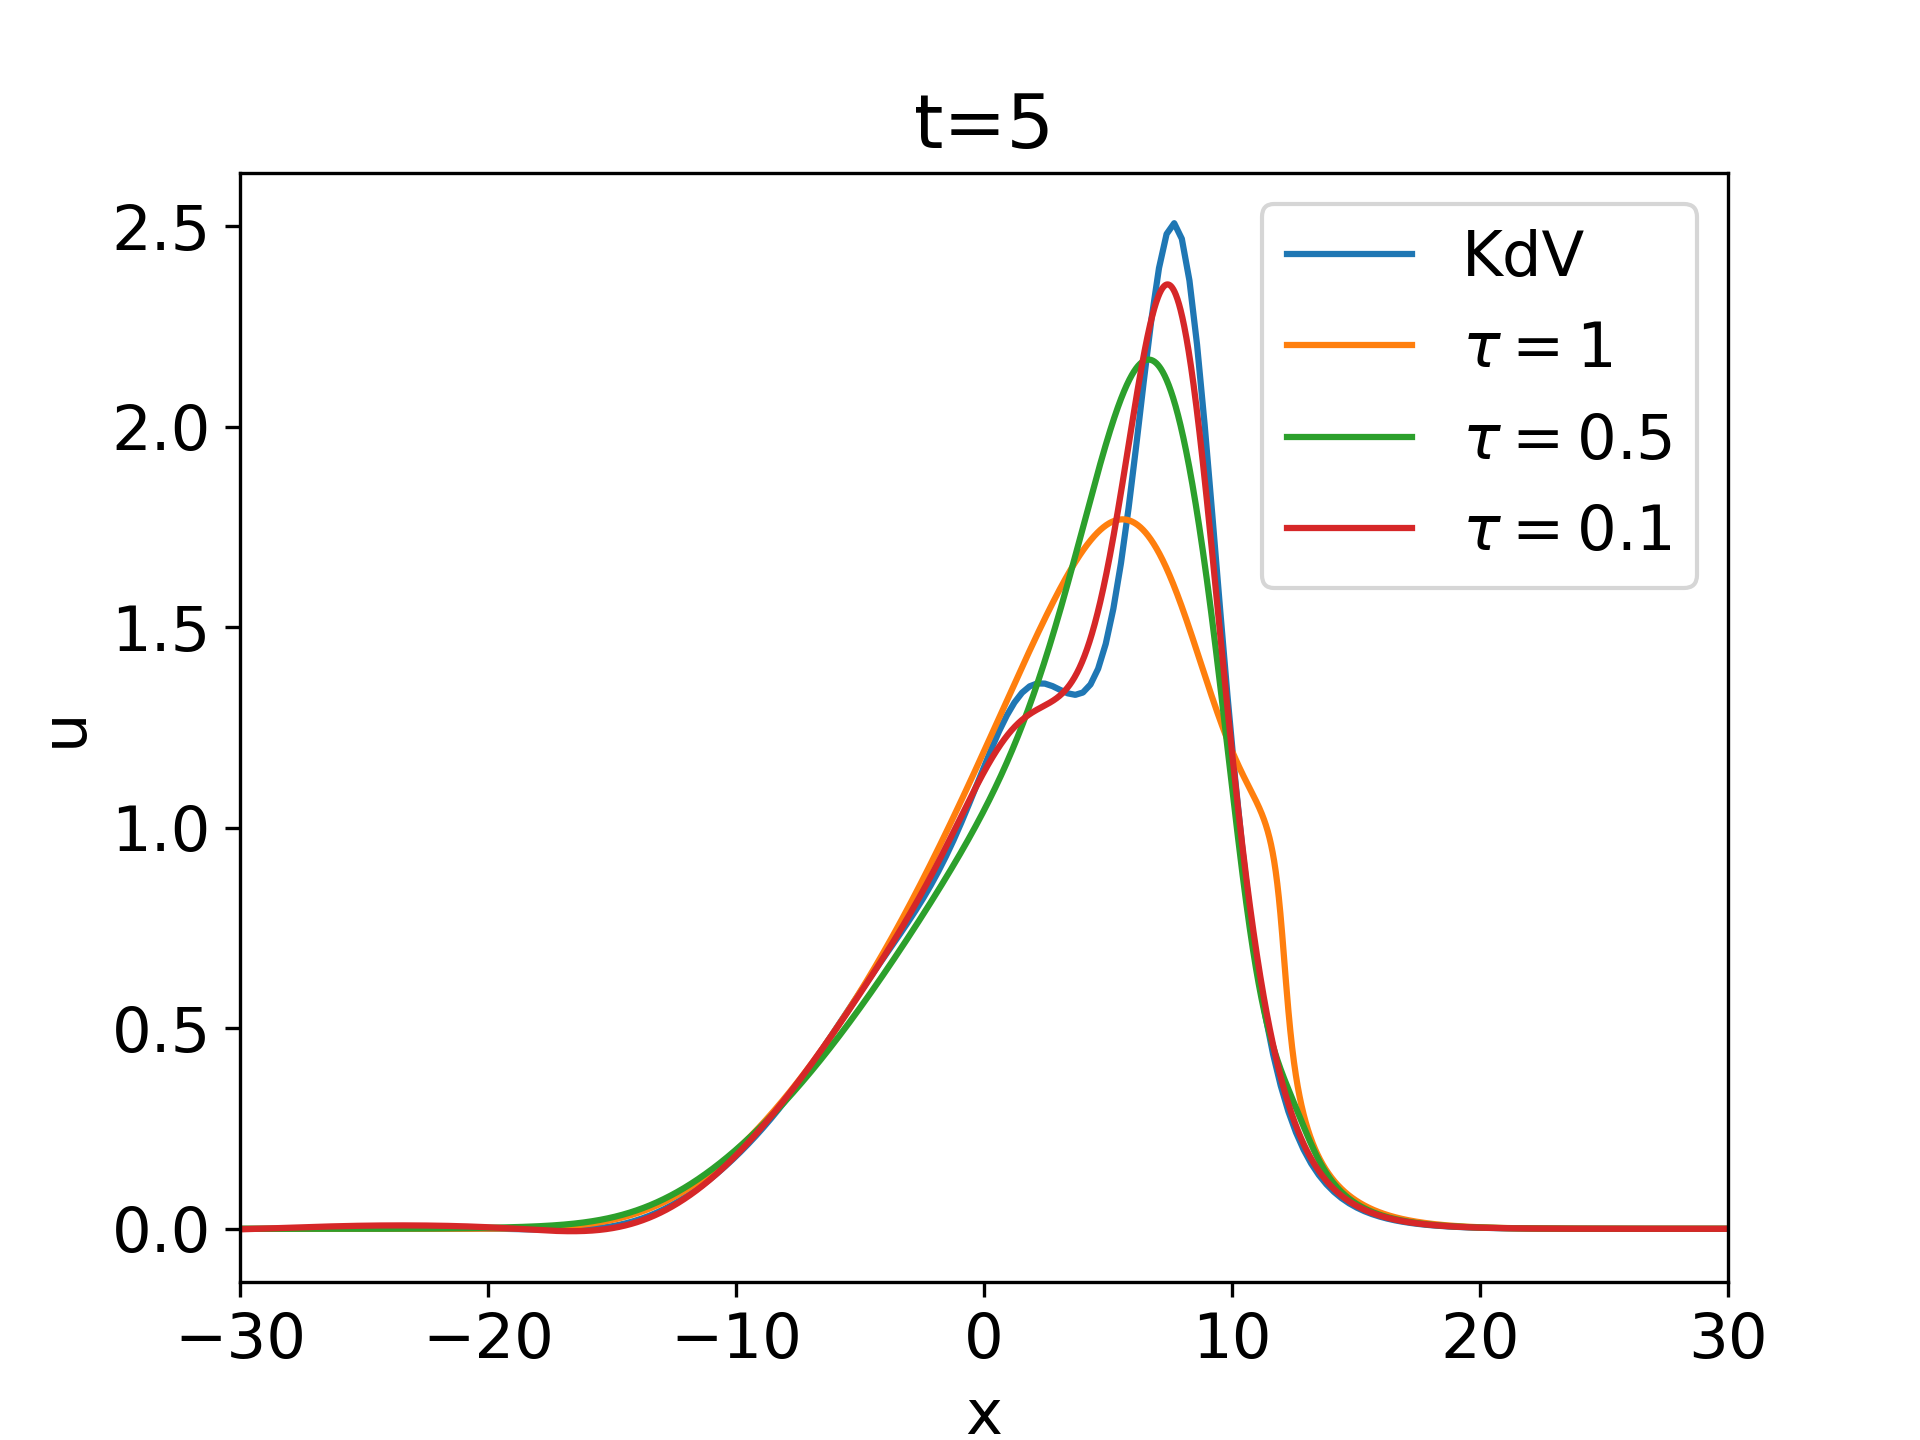
\includegraphics[width=4in]{figures/Convergence.png}
    \caption{Convergence of KdVH solutions to KdV.\label{fig:convergence}}
\end{figure}

In Figure \ref{fig:shocks}, we observe the clear appearance of shocks for $\tau=1$, while
the solution for $\tau=1/10$ is clearly devoid of shocks.

\begin{figure}
\centering
    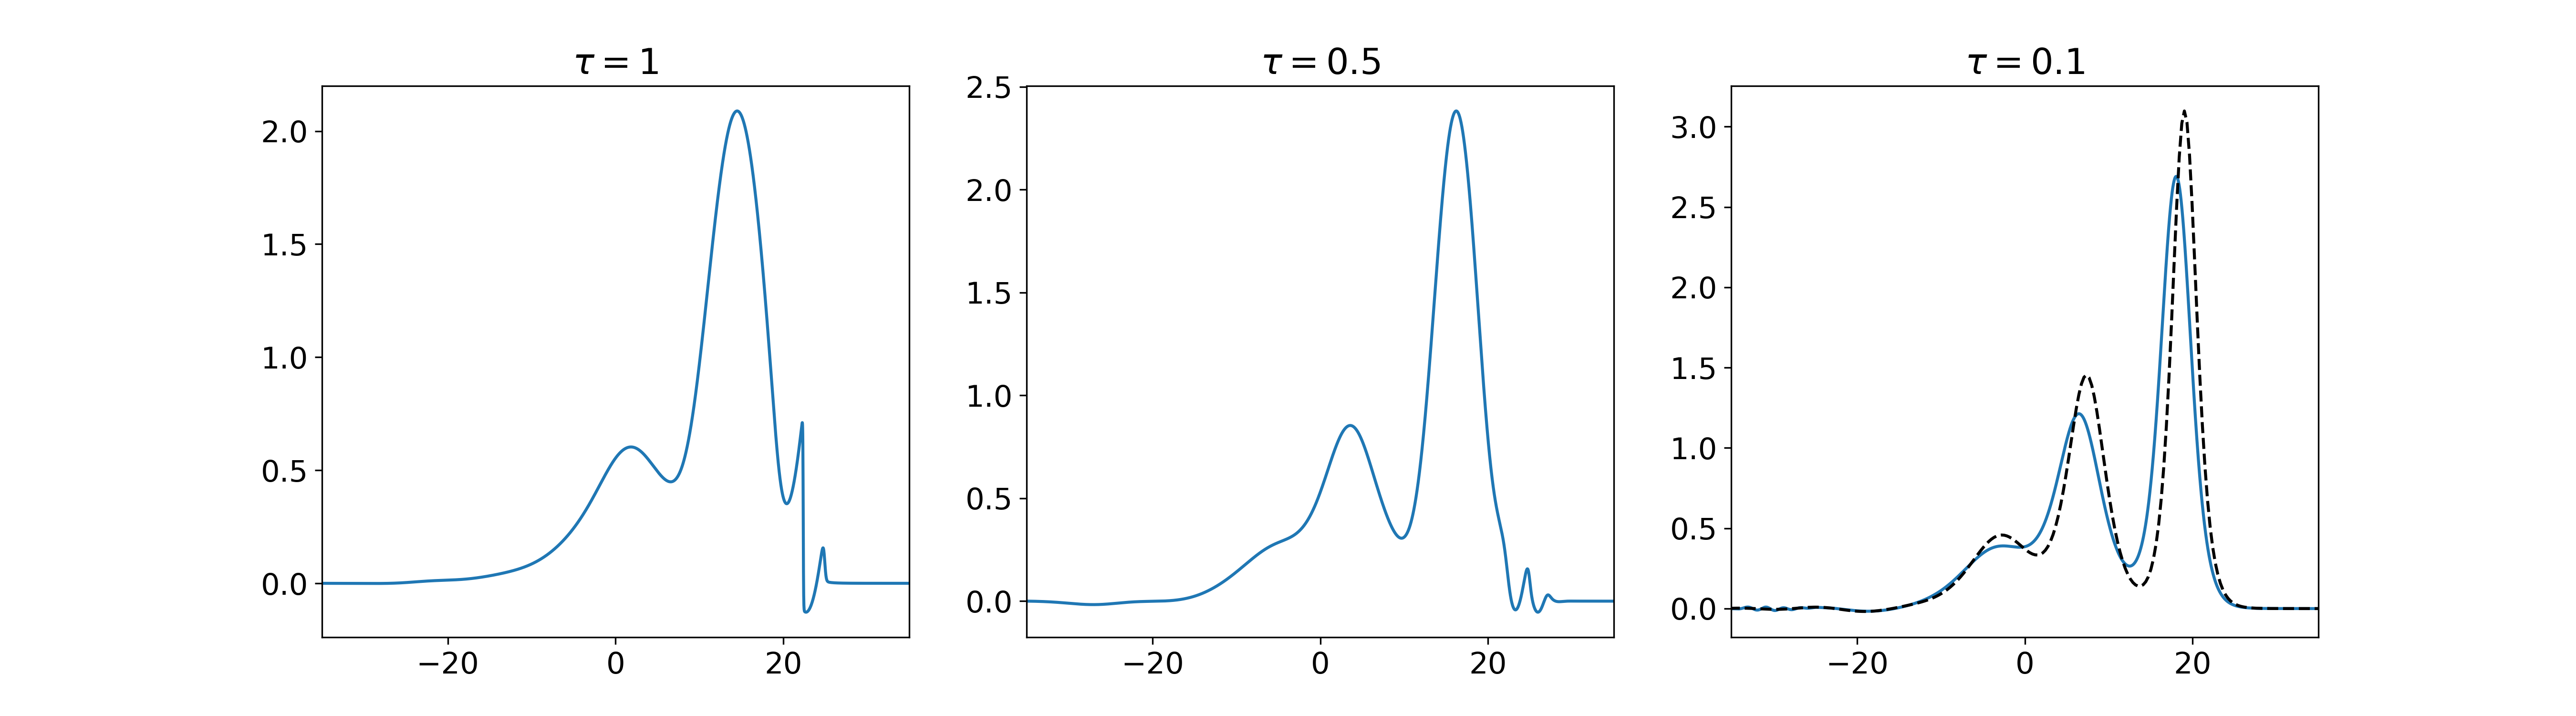
\includegraphics[width=6in]{figures/KdVH_solutions.png}
    \caption{Comparison of solutions at $t=16$.  In the last plot, the KdV solution is included (dashed black line)
    for comparison.\label{fig:shocks}}
\end{figure}


\todo{TODO}



\section{Summary and discussion}

\todo{TODO}



\appendix

\section*{Acknowledgments}

\todo{TODO: funding}
% \input{funding}


\printbibliography

\end{document}

